\chapter{利用数据提升} % Introduction chapter suppressed from the table of contents

Q:我每次都跑全量,引入低码平台,更多的是在需求设计阶段做好质量保证,
所以我们很注重量化质量管理,能否通过自动化来统计分析?
如何通过量化或工具方式实现自动评审?

A:为什么你觉得自动化会帮到你们?

Q:最近我们搞度量, 发现员工就会造数据, 结果导致失真,
度量哪里就造哪里, 所以还是想通过工具代替人工方式

A:现在我明白为什么你想自动化

Q:现在我们的主管很反感度量,一度量就有人造数据

A:度量本来是好的

Q:是的,就是大家知道算法原理就开始造假。
因为我们搞了红黑榜,很多人会想办法。

但很多人头脑都很聪明,但用于不合适的地方。

您的故事 验证了我度量与分析培训课都会分享的故事:

\framebox{%
\begin{minipage}[t]{0.97\columnwidth}\raggedright
利用数据提升管理

\begin{itemize}
\tightlist
\item
  某软件开发公司鼓励员工利用数据做过程改进,开始时很多成员不太接受但管理层一直支持坚持做下去
\item
  过了七个月,大家确实看到这种利用数据的过程改进使得团队质量跟生产率提升明显。
\item
  管理层觉得这个量化很成功,便把一些系数作为考核项,
\end{itemize}\strut
\end{minipage}}

猜猜会有什么后果。。。\\
后面团队的生产率就没有任何再提升了,
半年后,大家都觉得度量数据没有作用,管理层也不再用这些度量指标来考核了。

\textbf{度量主要是帮我们做分析找出根因做改进而不是仅仅为了监控}

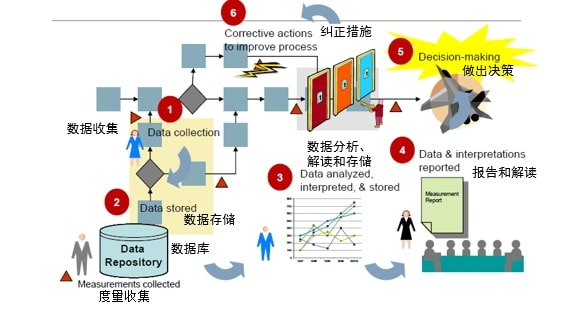
\includegraphics[width=10cm]{Ma4CarScreenshot_2021-12-27_205004.jpg}

\framebox{%
\begin{minipage}[t]{0.97\columnwidth}\raggedright
几十年前,我在企业做管理时,某一次花了三个月时间梳理一下工程的流程,大家都非常忙,都必须要自己加班加点腾出时间来做。\\
完成后,我便与大老板说``我们辛辛苦苦做了这些成绩可否公司给一些奖励?''\\
他便问我``我没看到你这次工程的流程梳理为公司增加了收入,公司没有额外收入,哪里有钱给你们奖励。''\\
我当时有点生气,但回想一下,他确实有道理。\strut
\end{minipage}}

Q:我们有很多数据统计分析,比如看测试用例与需求的比例。
其实客户发现的缺陷比例也降低了,但因为我们这行对质量特别注重,产品经过多年的逐步演化,过程很复杂,导致软件缺陷的修复很耗时,客户不太满意。\\
而且公司要求交付的频率要比以前高了很多,我们团队做这些分析都忙不过来,所以需要员工设自动化工具等加快速度才可以。

让我给你看看我们大数据分析。。。

A:我看好像你们是对所有项目的统计分析?

Q:是

A:你们管理者花精力分析数据出发点是好,但问题是团队会依赖你们管理者做分析
并非团队自己动脑筋持续改进。

Q:是的很多开发人员都觉得质量是你们(管理层)来管

A:你说的很好,这正是妨碍提升质量的最大障碍。
每个开发人员(甚至需求人员/产品经理)都要意识到质量好坏把握在自己手上,不能靠你们管理层或后面测试。
每次回顾要让他们把这些排除源头识别出来,他们才会感觉到自己的水平多差,前期遗漏了多少缺陷。

三十年前,Infosys
公司也是经历过这种过程,先让开发从数据发现很多缺陷都后期才被发现,导致大量返工。开发才有动力改进,把缺陷的发现提前,最终软件开发质量。
所以更快的自动化工具帮不了你们。

昨天与成都客户讲,要开始量化管理,不是自动化工具,而是个人,好比准备9个月后跑半马,必须锻炼和统计。

Q:你说的我都没想过,但觉得还是挺有道理的。

A:这点也是我昨天跟成都客户强调的:\\
\textbf{让所有员工改进整个系统问题}

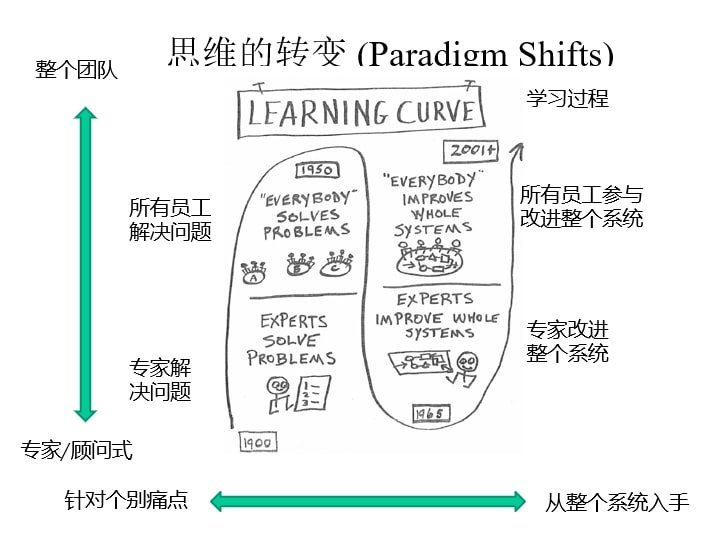
\includegraphics[width=10cm]{ImproveWholeSystemScreenshot_2021-12-27_204408.jpg}

总体的分析还有另一不足:各个项目特性不一样,你们现在几十个项目总体趋势分析,
很可能找不对根因,因每个项目的问题(根本原因)很可能不同。
比如,同样是一个测试用例比例数,你的范围就很宽 -
从最低的0.3到最高的超过200!但你们取平均值5.1 来做分析。

收集数据也是问题,因收集数据是挺花精力的工作

Q:完全100\%同意

答:但正因为不同项目有各种特性,要对收集到的数据做分析也很耗时。
这些辛辛苦苦做出来的分析报告其实不仅仅是给高层(或者项目经理),
在每一个团队成员都看到才有意义
。(度量分析要反馈回数据提供者,他们才有动力继续收集数据)要把那些分析好的报告再跟每一个团队成员解释上要花多大精力?

如果把数据分析下放到团队自己搞,便灵活很多了;也正因为他们有参与收集和分析讨论,
你们也可以节省很多沟通的成本。

所以你们领导应该定位自己是内部老师,辅导团队怎么做好数据分析,效果会更好。

Q:就当团队自己讨论便可以得到改进吗?不需要我们领导?\\
答:只要他们有一个较高的目标,不要低估人的潜力,只要他感觉到现状跟目标有差距,他也想挑战自己,达到这个高的目标。最近看一个电视节目播放三个滑翔伞者挑战海拔6250米幺妹峰的过程,他们都很有经验,装备齐全,比如贴在鼻子供氧的设备等等。他们一直观察天气情况,因为滑翔伞必须要借用上升的气流才可以上升。其中一位一直观察小鸟飞行,就选择鸟的方向去飞,确实有一股上升气流,中间经过如大雾,差点撞上山等惊险过程,最终完成,他开心极了(详见附件)。\\

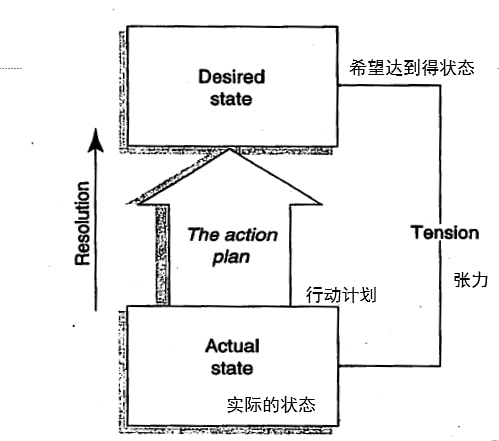
\includegraphics[width=10cm]{Tension2ImproveScreenshot_2021-12-27_204553.jpg}

希望达到的状态,就可以克服种种困难,团队也一样,如果有很高的目标,都会想办法,尽力完成,人的智慧无限,领导要相信团队的潜力。所以我们说度量就是让他们可以实际看到目标与现状的差距。具体怎么做?他们最清楚。刚才滑翔伞的案例,是否可以有一个经验丰富的远程教练教他们怎么做?不可能,都是要靠现场的经验,依据实际的情况去寻找合适的机会,有可能成功,有可能失败。\\
希望团队提升,达到那个最高目标也一样,不可能有一套所有团队适用的方法。我们作为领导主要是作为一个教练支撑他怎么去做,最终还是要靠自己。团队的成长跟一个小孩的一样。比如你看见现在年轻的父母,也可能是当一个小孩。不让他自己走路而坐学步车,不让他自己吃饭而喂他,你估计他后面可以独立成长吗?这样会造成过度依赖,对成长不好。\\
Q:你说都是个人提升例子,整个公司提升就没你说这么简单。\\

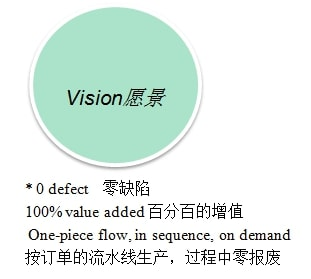
\includegraphics[width=10cm]{远景1.jpg}

A:是的,但道理还是一样,比如你看看上面这个图。假设你是50年代的一家汽车公司,你的销量、成本、效率就那些先进的世界级汽车公司差很远。你觉得能达到图中这个零缺陷、零废物、一次性流水线生产目标吗?\\
问:不太可能,所有过程都有极限,到了一定程度就无法再提升了。\\
答:现代的汽车生产过程差不多可以达到上以上的水平,刚才我说的就是现在世界最大的汽车公司丰田。当时他觉得美国汽车公司那种依据福特的生产线做法,不能适应不同客户的定制需求,而且从原材料到生产出汽车很慢,他就一直研究如何达
Just In Time
目标。现代,5、60年后,这种生产方式已成为世界级的标准生产流程,如英国牛津日产为德国宝马公司生产魅影汽车的生产线,可以做到每个步骤都没有多余的库存;
而且从原材料(钢材)到完成生产出汽车只需要24小时。\\
Q:如何激发团队战斗力,是否有一些建议和方法?\\
听你的故事,每次迭代量化目标要由团队自主分析,设定,怎样做?

A:问得好,很多想利用敏捷开发做提升的公司也问。
我在下一篇"量化质量管理FAQ"里有解答您这问题。\\
大家可能也遇到类似的困惑,后面会先分享一些案例,然后用问答形式解读这些方法如何能解决以上问题。本章用以下故事总结:

\framebox{%
\begin{minipage}[t]{0.97\columnwidth}\raggedright
\begin{itemize}
\tightlist
\item
  新上任的总监很了解前期评审的重要性,他发现团队一直都没有评审的习惯,并下令所有项目必须要做评审,而且要把评审的数字定期上报。总监为了鼓励团队做评审,也对评审效果做了一些奖励措施。所以每次在月会上,总监都会听到团队关于评审的记录、报告。\\
\item
  但其实他不知道的是,团队实际上没有做任何评审,可能只是在酒吧聊天的时候,随便写一些出来变成报告上交。后面总监终于发现真相,非常生气。\\
\end{itemize}\strut
\end{minipage}}

\textbf{经验教训}:

\begin{itemize}
\tightlist
\item
  单靠上层制定方法,下面不明白为什么要做这件事,只是听指挥去执行,往往得不到什么改进效果。改进必须是源自团队本身才可以持久。更应参照XY理论,让团队自发解决问题,并提升。
\item
  只优化了某一个过程,不一定能改进整个系统,必须``所有人参与改进整个系统''。在复盘时,让团队回顾冲刺数据,并一起讨论如何在下轮冲刺改善。
\end{itemize}

\hypertarget{ux9644ux4ef6ux9996ux4f4dux901aux8fc7ux65e0ux52a8ux529bux6ed1ux7fd4ux4f1eux98deux8d8aux5e7aux59b9ux5cf0ux6d77ux62d46250ux7c73ux7684ux4eba}{%
\subsection{附件:首位通过无动力滑翔伞飞越幺妹峰(海拔6250米)的人}\label{ux9644ux4ef6ux9996ux4f4dux901aux8fc7ux65e0ux52a8ux529bux6ed1ux7fd4ux4f1eux98deux8d8aux5e7aux59b9ux5cf0ux6d77ux62d46250ux7c73ux7684ux4eba}}


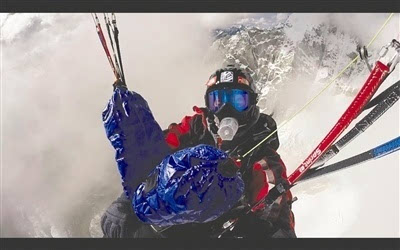
\includegraphics[width=10cm]{滑翔2.jpg}

飞行中的李群国\\

\begin{itemize}
\tightlist
\item
  2016年,34岁的李群国以6356米的高度环绕幺妹峰峰顶一圈\\
\end{itemize}

10月18日,一支三人飞行团队在四川阿坝州四姑娘山完成了一次极具挑战的探险:他们用无动力滑翔伞的方式飞越了海拔6250米素有``蜀山皇后''之称的幺妹峰。其中,34岁的李群国经过2小时40分的飞行,以6356米的高度在环绕峰顶一圈后,顺利返航。\\
\textbf{挑战}\\
云终于散开了一点!10月18日中午12时,在位于四姑娘山南侧海拔3950米的朝山坪,李群国和他的队友------中国滑翔伞国家队教练元林朝、中国越野飞行记录保持者宋俊明三人齐齐地望向远处。``应该差不多了。''元林朝转过身,招呼着现场的人员做好飞行前的最后准备。\\
他们的目标正是眼前的这座雪山------素有``蜀山皇后''之称的四姑娘山幺妹峰。在这之前,他们已经等候了近三个小时。\\
最先起飞的是宋俊明。要想让滑翔伞持续升空,必须依靠上升气流的辅助,但宋俊明经数次寻找,最终还是没能找到上升气流,只得放弃飞行,安全降落。而此时,天气再次被云雾笼罩。元林朝和李群国只好继续等待时机,期望天气好转。\\
一个小时后,转机再次出现,元林朝和李群国决定再冒险一试,于是,两人先后起飞。``恰好就碰到了好运气。''李群国介绍,飞出不久,就遇上了一股上升气流,高度慢慢爬升到了4800米。接着两人尝试着靠近第一座大妹峰,靠近后又遇到了下一股上升气流,便继续往二三妹峰靠近,看起来一切都很顺利。\\
~\\
不过,在靠近幺妹峰时,峰顶再次出现了云雾。``云雾里飞行好比大雾里开车一样,是极其危险的。''尽管已经飞至6100米高度,元林朝经过判定,还是选择了返航。但此时的李群国却冒了一把险,凭着气流继续上升,并成功越过了幺妹峰,``当时就是想突破一下,虽然确实有些冒险,但我们成功了,这个团队成功了。''\\
\textbf{惊险}\\
上升途中突遭下沉气流,瞬间下跌100米\\
其实,李群国的成功飞越同样伴随着惊险。用他自己的话说,``像是一场玩命,但决定了要去挑战,就已经有了心理准备,探险都有可能付出代价,哪怕是生命。''\\
就在李群国过了三妹峰时,他遭到了一股下沉气流,高度重新下降到了4800米左右,``这个时候有可能就找不到机会再攀升了。''于是,他调整了飞行方式,绕到了幺妹峰的西北角,准备降落。而就在降落的过程中,又再次遇到了一股很强的上升气流,他内心一阵暗喜,高度又迅速地上升到了5500米左右。\\
然而,这股强大的上升气流却也伴随着致命的危险。``往往在强上升气流的边缘就会伴随着强下沉气流,一旦遇上了就会非常快速地往下掉,尤其是在高原地区,气流的复杂程度更大。''李群国说,而自己却正好遇上了这股伴随的强下沉气流。\\
突然间,李群国就失去了动力,伞翼出现变形,整个人和滑翔伞开始不正常地下降,伴随着旋转和俯冲,做着自由落体运动。``一瞬间的工夫,就掉下了100多米。''好在对于已经从事滑翔伞飞行达15年的他来讲,这样的情况仍在他的控制范围内。经过一系列的调整,才最终恢复正常飞行。\\
李群国最后的飞行高度达到了6356米,超出顶峰达100多米,而此时眼前的云雾也为他打开了一扇窗,云缝里的幺妹峰让他激动不已,``太震撼,已无法用言语表达。''\\



